\onecolumn
\section{Tabellen, Anhänge}
% \begin{center}
%     Wichtig: in Farbe ausdrucken!
% \end{center}
% \centering
\large
\textbf{F39 - Gleichstromwiderstand, Seildurchmesser, Sollquerschnitt (Freileitung)}

\centering
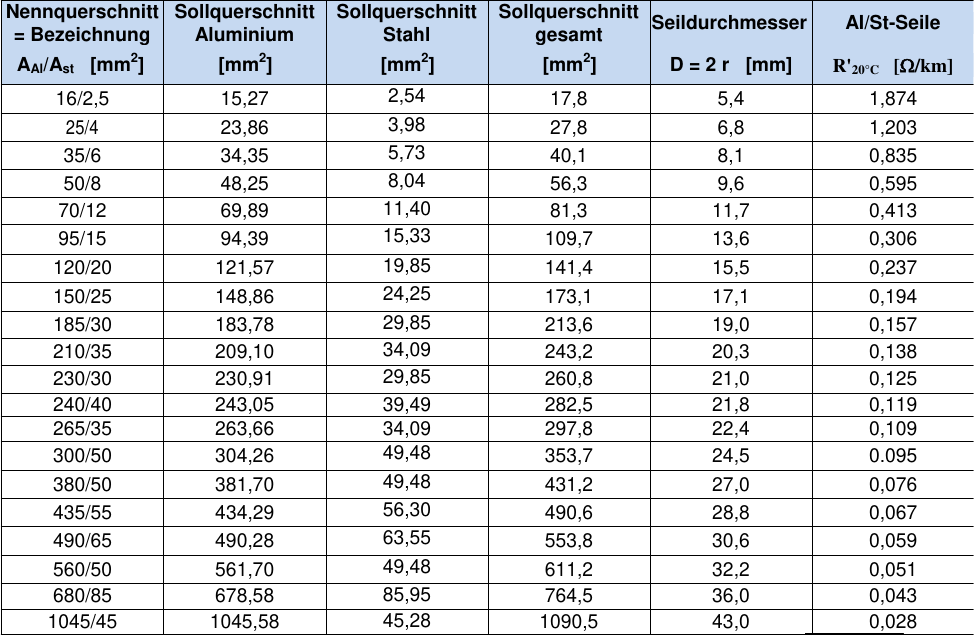
\includegraphics[width=0.9\columnwidth]{figures/freileitung_f39_resistanzbelag.png}

\raggedright
\textbf{F42 - Widerstandserhöhung durch Skineffekt (Freileitung, Kabel)}

\centering
\includegraphics[width=0.9 \columnwidth]{figures/f_42_widerstandserhöhung_skineffekt.png}

\raggedright

\newpage
\textbf{F43 - Resistanzbelag, Richtwerte Seilbelegungen (Freileitung)}

\begin{center}
\begin{tabular}[h]{|c|c|c|}
    \hline
    Leitung $[kV]$ & Seiltyp & $R'_b \left[ \frac{\Omega}{km} \right]$ \\
    \hline
    10/20 & Einfach& 0,3 - 0,6 \\
    \hline
    110 & Einfach& 0,2 - 0,15\\
    \hline
    220 & Zweierbündel& 0,09\\
    \hline
    380 & Viererbündel & 0,03\\
    \hline
\end{tabular}
\end{center}

\textbf{F46 - Reaktanzbelag, Richtwerte Hochspannungsleitungen (Freileitung)}

\makebox[\textwidth][c]
{
\begin{minipage}{0.5\textwidth}
\begin{tabular}{|c|c|}
    \hline
    Seiltyp & $X'_b \left[ \frac{\Omega}{km} \right]$ je Leiter \\
    \hline
    Einerseil & 0,40 \\
    \hline
    Zweierbündel & 0,30 \\
    \hline
    Viererbündel & 0,23 \\
    \hline
\end{tabular}
\end{minipage}
\hspace{-5em}
\begin{minipage}[c]{0.5\textwidth}
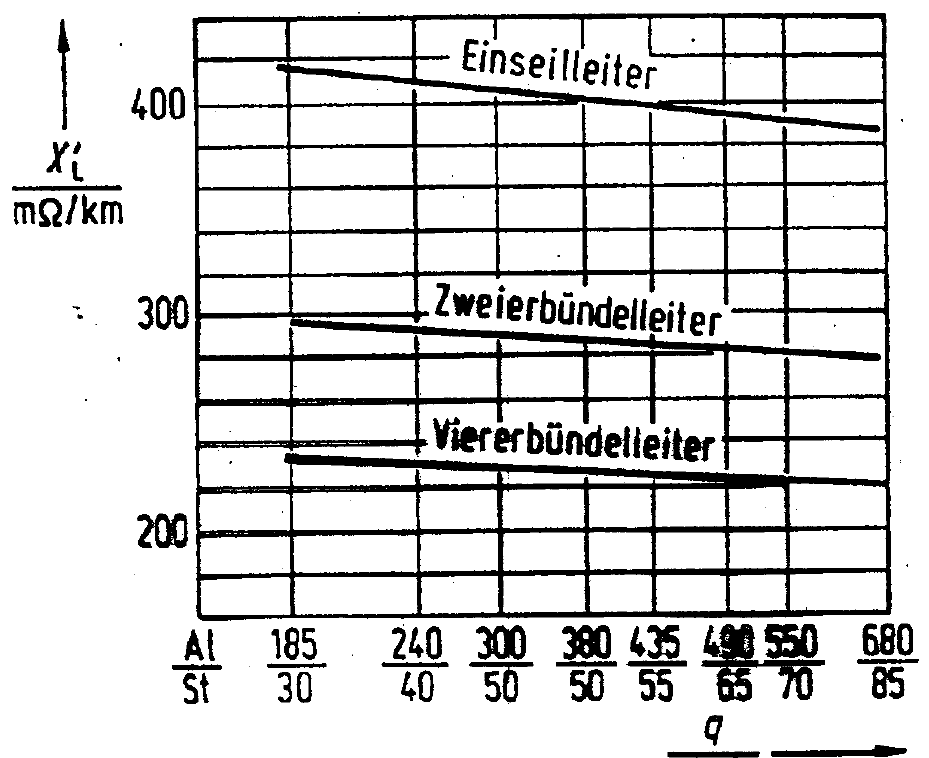
\includegraphics[width=\columnwidth]{figures/f46_freileitung_reaktanzbelag.png}
\end{minipage}
}

\textbf{F48 - Suszeptanzbelag, Richtwerte Einfachseil bei f=50Hz (Freileitung)}

\makebox[\textwidth][c]
{
\begin{minipage}{0.5\textwidth}
\begin{tabular}{|c|c|}
    \hline
    Richtwerte $U_{Betrieb}$ & $B'_b \left[ \frac{\mu S}{km} \right]$ je Leiter \\
    \hline
    < 30 kV & 3,5 \\
    \hline
    > 30 kV & 3 \\
    \hline
\end{tabular}
\end{minipage}
\hspace{-5em}
\begin{minipage}[c]{0.5\textwidth}
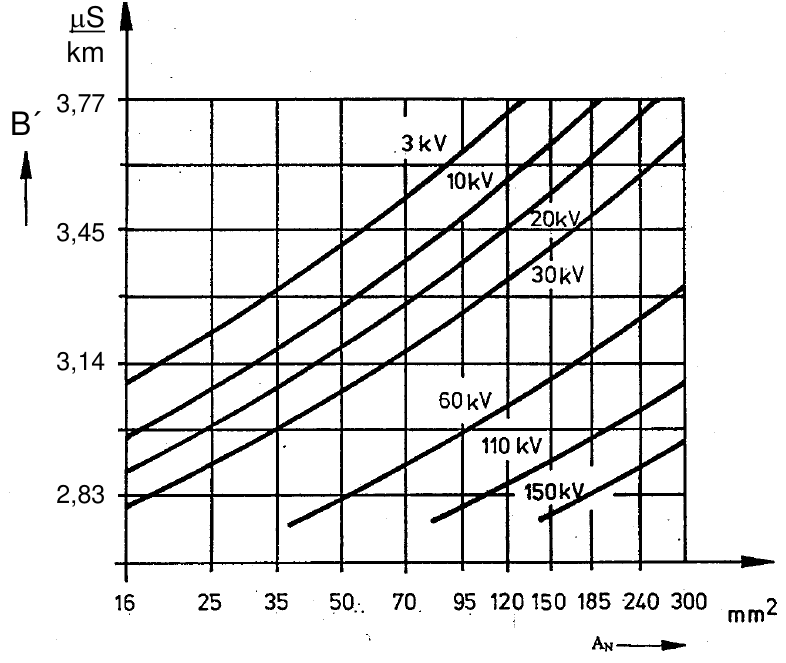
\includegraphics[width=\columnwidth]{figures/f_48_freileitung_suszeptanzbelag.png}
\end{minipage}
}

\textbf{F49 - Konduktanzbelag, Richtwerte (Freileitung)}

\makebox[\textwidth][c]
{
\begin{minipage}{0.5\textwidth}
\begin{tabular}{|c|c|}
    \hline
    Richtwerte $U_{Betrieb}$ & $G'_b \left[ \frac{nS}{km} \right]$ je Leiter \\
    \hline
    < 30 kV & vernachlässigbar \\
    \hline
    110 kV & 4 - 5 \\
    \hline
    220 kV & 2,5 - 3,5 \\
    \hline
    380 kV & 1 - 2\\
    \hline
\end{tabular}
\end{minipage}
\hspace{-5em}
\begin{minipage}{0.5\textwidth}
\begin{itemize}
    \item Strom über Isolation (hier Luft) gegen Erde
    \item Ursachen: Korona- und Isolationsverluste
\end{itemize}
\end{minipage}
}

\newpage


\textbf{F34 - Resistanzbelag $\mathbf{R'_{=}}$ in $\mathbf{\frac{\Omega}{km}}$ (Kabel)}

% \makebox[\textwidth][c]
% {
% \hspace{-5em}
% \begin{minipage}[c]{0.5\textwidth}
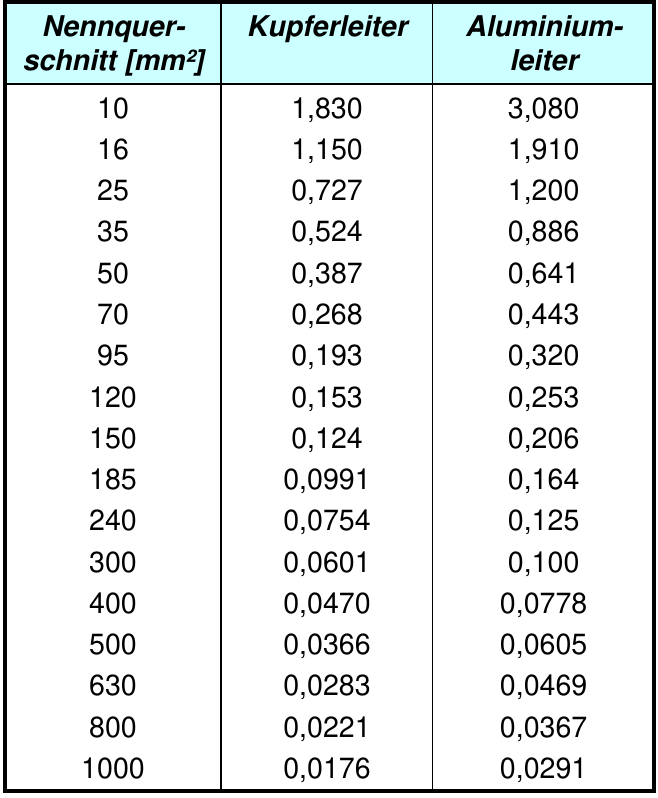
\includegraphics[width=0.35\columnwidth]{figures/f34_Kabel_Gleichstromwiderstand.png}
% \end{minipage}
% }

\textbf{F37 - Widerstandserhöhung durch Proximityeffekt $\mathbf{F_P}$ (Kabel)}

% \vspace{-10pt}
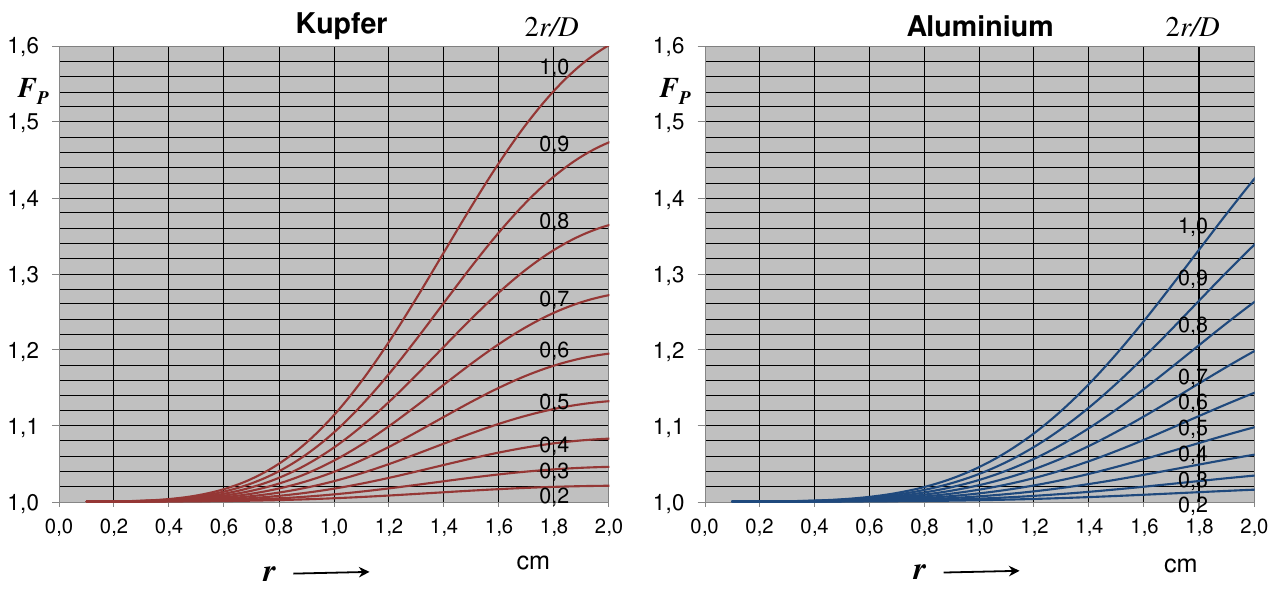
\includegraphics[width=0.9\columnwidth]{figures/F37_Kabel_Resistanzbelag_Proximityeffekt.png}


\textbf{F42 - Verlustfaktor/$\mathbf{\varepsilon-}$Konstante von Isolierstoffen (Kabel)}

\centering
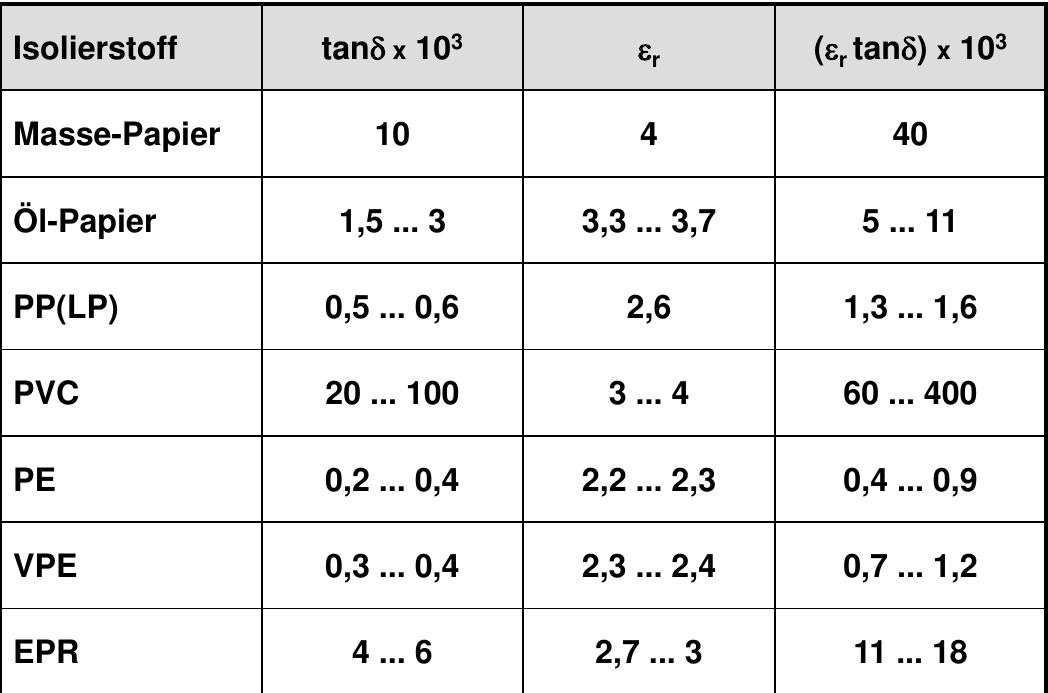
\includegraphics[width=0.5\textwidth]{figures/f42_verlustfaktor_e-konstante_isostoffe.png}

\raggedright
\textbf{F40 - Reaktanzbelag $\mathbf{X'_b}$, Richtwerte (Kabel)}

\centering
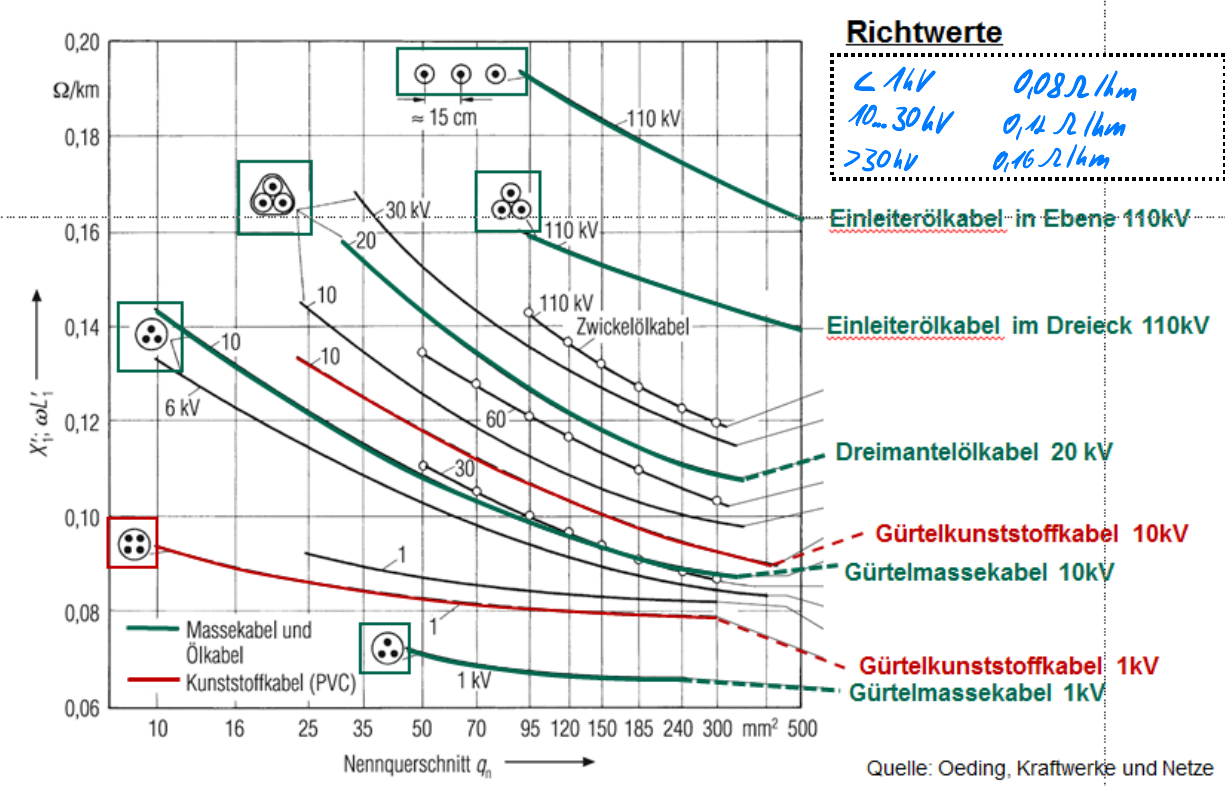
\includegraphics[width=0.7\columnwidth]{figures/f39_reaktanzbelag_kabel.png}

\raggedright
\textbf{F43 - Suszeptanzbelag $\mathbf{B'_b}$ - Richtwerte Radialfeldkabel mit Masseisolierung $\varepsilon_r = 4$}

\centering
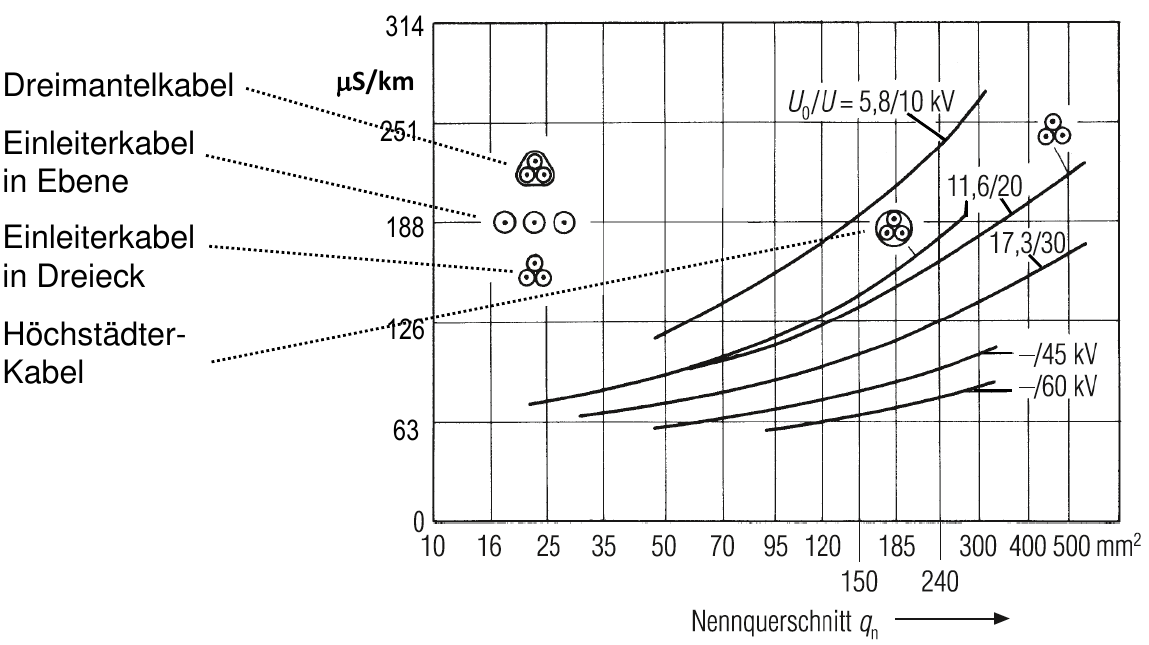
\includegraphics[width=0.7\columnwidth]{figures/f43_kabel_radialfeldkabel_masseiso.png}

\raggedright
\textbf{F44 - Suszeptanzbelag $\mathbf{B'_b}$ - Richtwerte (Kabel)}

\centering
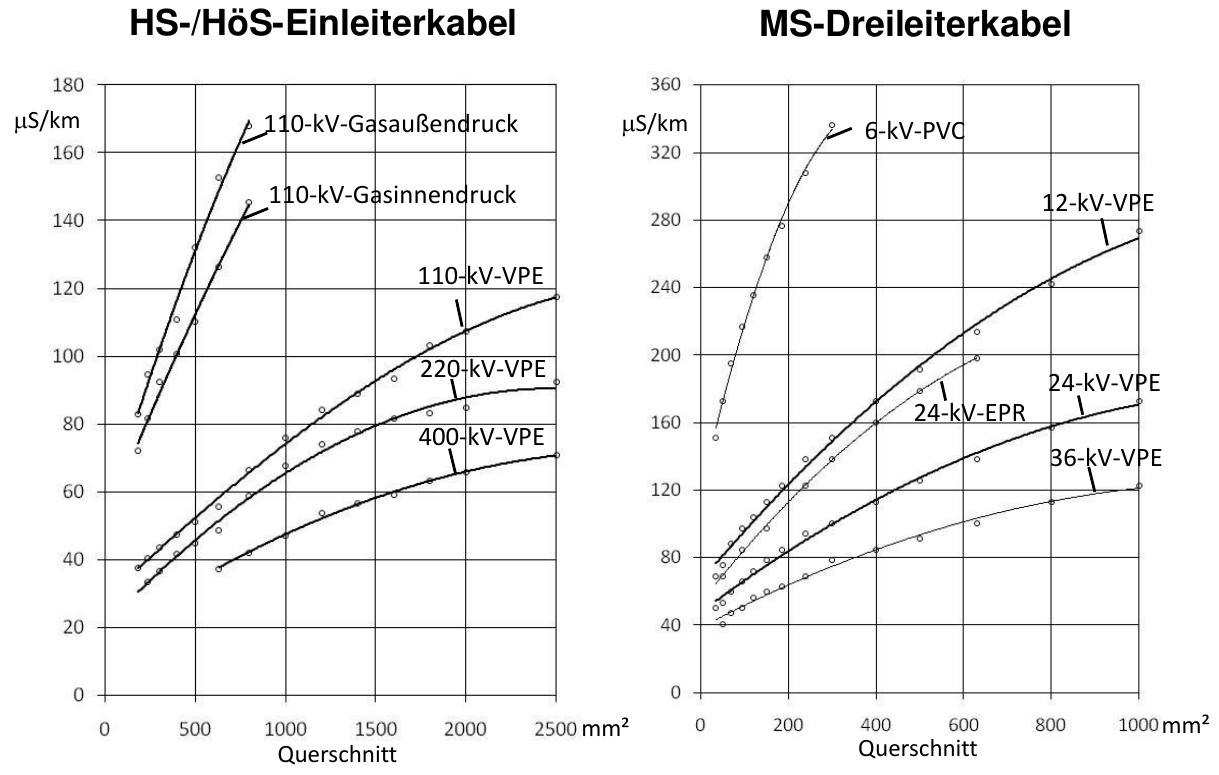
\includegraphics[width=0.6\textwidth]{figures/f44_suszeptanzbelag_weitere_kabeltypen.png}

\raggedright
